\begin{task}{4, Fire Evacuation Planning for the MI Building}
In response to the increasing student population at the Technical University of Munich, there is a pressing need to reassess the fire evacuation plan for the MI building (Figure \ref{MI-building}). To address this, an experiment was conducted where the fire department tracked 100 random students and employees on different days during the busiest hours to obtain data on the distribution of people within the MI building, denoted as \(p(x)\). The primary objective of the initial experiment was to estimate the number of people in a critical area of the building, marked by the orange rectangle in front of the main entrance, ensuring that it does not exceed 100 people. The experiment is divided into several steps, including data visualization, training a Variational Autoencoder (VAE) on the FireEvac dataset, visualizing the reconstructed test set, generating samples, and estimating the critical number of people. This series of experiments aims to gain a deep understanding of the distribution of people within the MI building through machine learning and simulation, providing robust support for the optimization of the fire evacuation plan.

\begin{figure}[H]
\centering
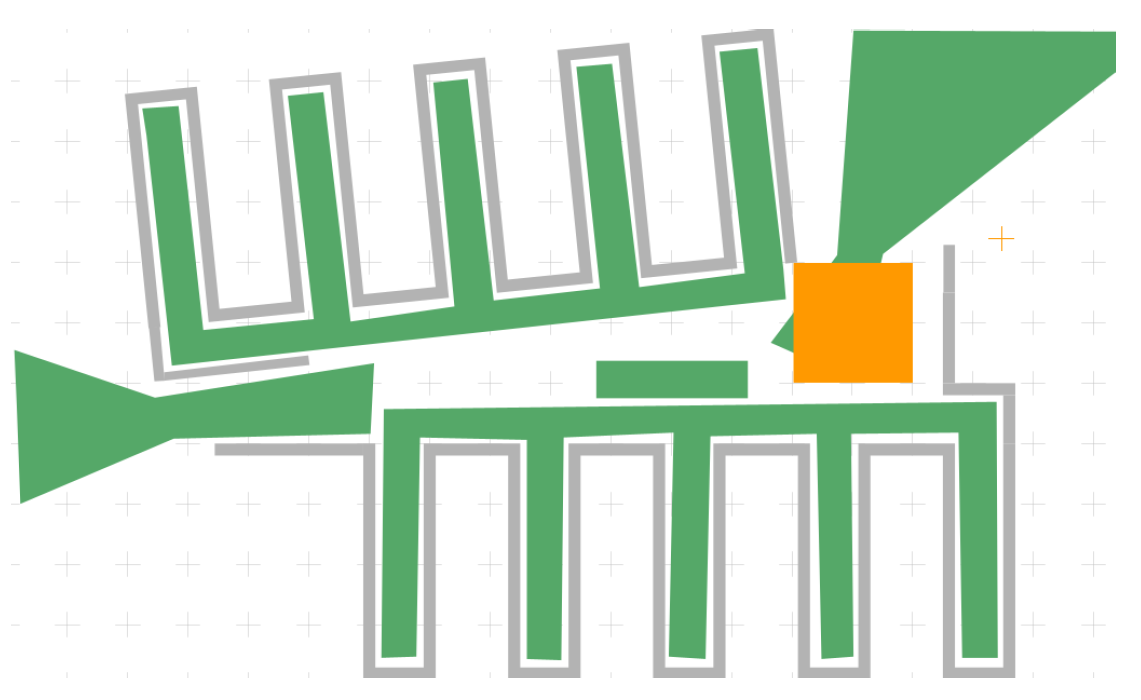
\includegraphics[width=0.5\textwidth]{images/MI_building.png}
\caption{Schematic of the MI building in Garching}
\label{MI-building}
\end{figure}


\paragraph{Visualise FireEvac Dataset}
To effectively visualize the data points in the FireEvac Dataset, we have plotted them as scatter points in Figure \ref{FireEvac_visualization}. There are 3,000 training data points, represented in blue, and 600 testing data points, represented in red.

\begin{figure}[H]
\centering
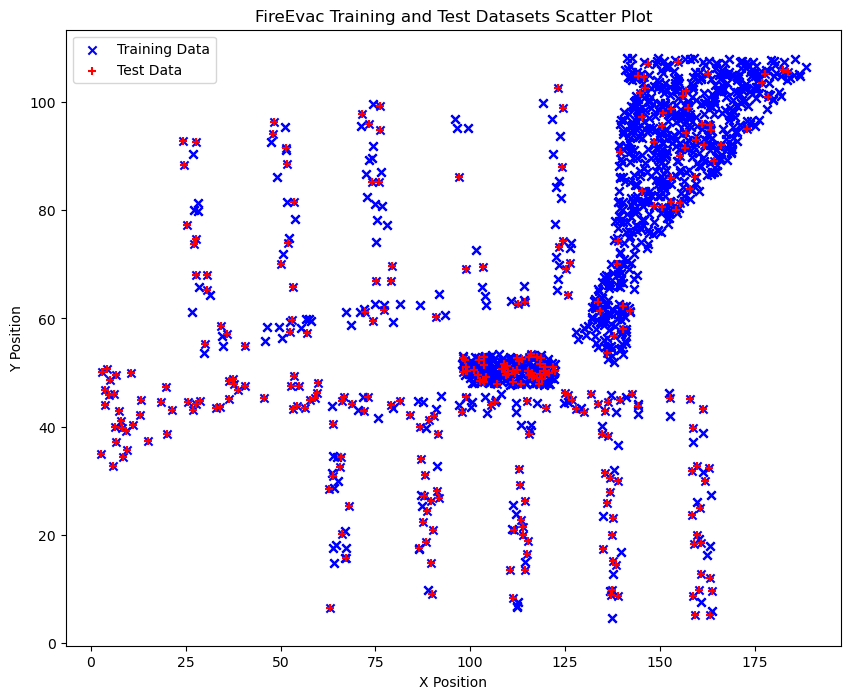
\includegraphics[width=0.6\textwidth]{images/FireEvac_visualization.png}
\caption{FireEvac Training and Test Dataset Scatter Plot}
\label{FireEvac_visualization}
\end{figure}

\paragraph{VAE traning on FireEvac Dataset}
In order to learn the probability distribution \( p(x) \) on the FireEvac dataset, a Variational Autoencoder (VAE) was trained. The VAE implementation used in this task was adapted from Task 3, with adjustments made to the number of input and output neurons, and varying the number of layers. However, after some hyperparameter tuning, we changed the model slightly. In particular, we changed the activation function of the hidden layers from ReLU to LeakyReLU(0.2). Using the ReLU activation function the reconstructed results were very bad due to abruptly transforming negative inputs to 0. With the LeakyReLU we got a smooth transition when getting negative inputs and weights. The new model can be found in \verb|model_fire_evacuation.py| with the only change being the replacement of the activation function. 

To enhance model performance and take advantage of the sigmoid function in the decoder, the input data \( x \) was rescaled to a range of \([0, 1]\) before initiating the training process. For the architecture of the VAE, a configuration of 2-64-64-2 neurons for the encoder and decoder was employed. This translates to a two-dimensional latent space and two hidden layers, each comprising 64 neurons. The chosen learning rate was 0.005, utilizing the Adam optimizer with a batch size of 64. The model underwent training for 200 epochs. 

Due to our loss being composed of two components, likelihood and KL-loss, where the KL-loss incorporates a scaling factor \(\beta\), the loss is defined as \( \text{loss} = - \text{likelihood} + \beta \times \text{kl\_loss} \). Because the performance of the trained model varies under different \(\beta\) parameters, we trained models with \(\beta\) values of 0, 0.5, and 1 to perform the following tasks.



\paragraph{Reconstructed Test Set}
The performance of the model in reconstructing the test dataset under three different \(\beta\) values is illustrated in Figure \ref{fig:beta}. When \(\beta\) is set to 0, the VAE degrades into an AE, and it almost perfectly reconstructs the test dataset, as depicted in Figure \ref{fig:beta0}. This happens because the input dimension and the latent space dimension is the same, 2, so the latent space basically copies the distribution of the points in the original data, learning the trivial encoding. For \(\beta = 0.5\) , although there is a slight deviation between the reconstructed data and the original data, it essentially captures the pattern of the test dataset, as shown in Figure \ref{fig:beta05}, as the regularizer KL is weak. When \(\beta\) is set to 1 \ref{fig:beta1}, the distribution of the reconstructed data is more dispersed compared to the original data, as the encodings are forced to be closer, breaking the trivial encoding. Therefore, the VAE is forced to learn a 2-d encoding closer to the prior distribution, of 2-d data points, a process that is quite inefficient. It is noteworthy that in this case, in the top right corner, the distribution of the reconstructed data forms a line, which is not ideal.

We can observe the differences in the latent space in Figure \ref{fig:betalatent}. We can note with \(\beta = 0\) how the model tries to learn a trivial encoding imitating the distribution of the 2-d datapoints, whereas with \(\beta = 1\) the latent space is constrained by KL so it learns an unprecise trivial representation of the datapoints, without finding an efficient encoding that is actually able to compress the information and reconstruct it. This is mainly because the input data already has a dimension of 2.


\begin{figure*}[ht]
\centering

\subfigure[\(\beta=0\)]{
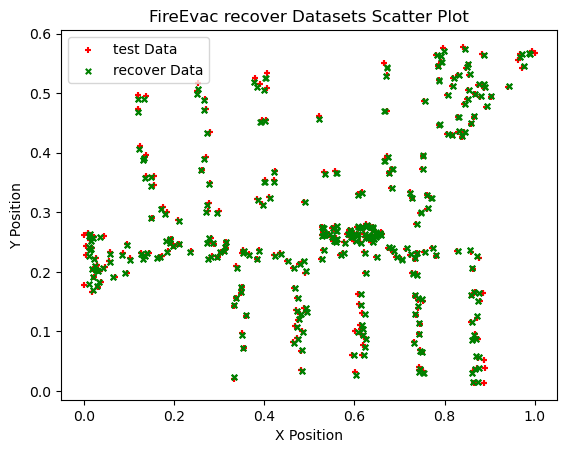
\includegraphics[width=0.3\textwidth]{images/recover_test_beta0.png}
\label{fig:beta0}
}
\hfill
\subfigure[\(\beta=0.5\)]{
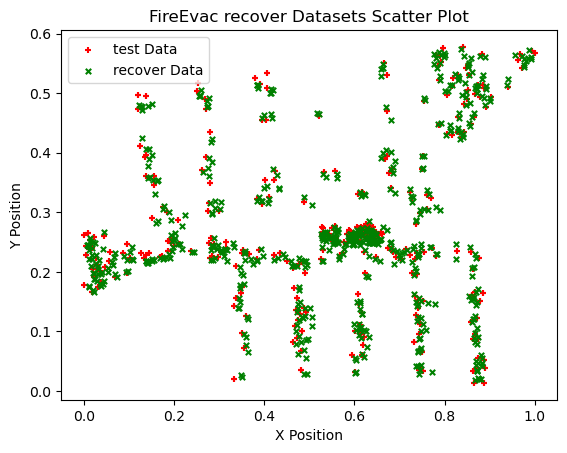
\includegraphics[width=0.3\textwidth]{images/recover_test_beta0.5.png}
\label{fig:beta05}
}
\hfill
\subfigure[\(\beta=1\)]{
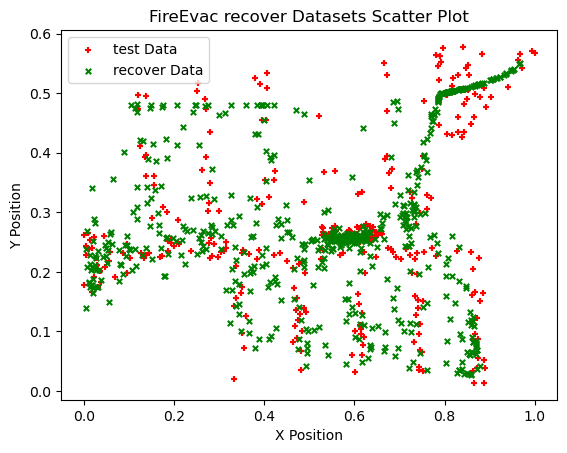
\includegraphics[width=0.3\textwidth]{images/recover_test_beta1.png}
\label{fig:beta1}
}

\caption{Reconstructed Test Set for Different \(\beta\) Values}
\label{fig:beta}
\end{figure*}


\begin{figure}[ht]
\centering
\subfigure[Latent space \(\beta=0\)]{
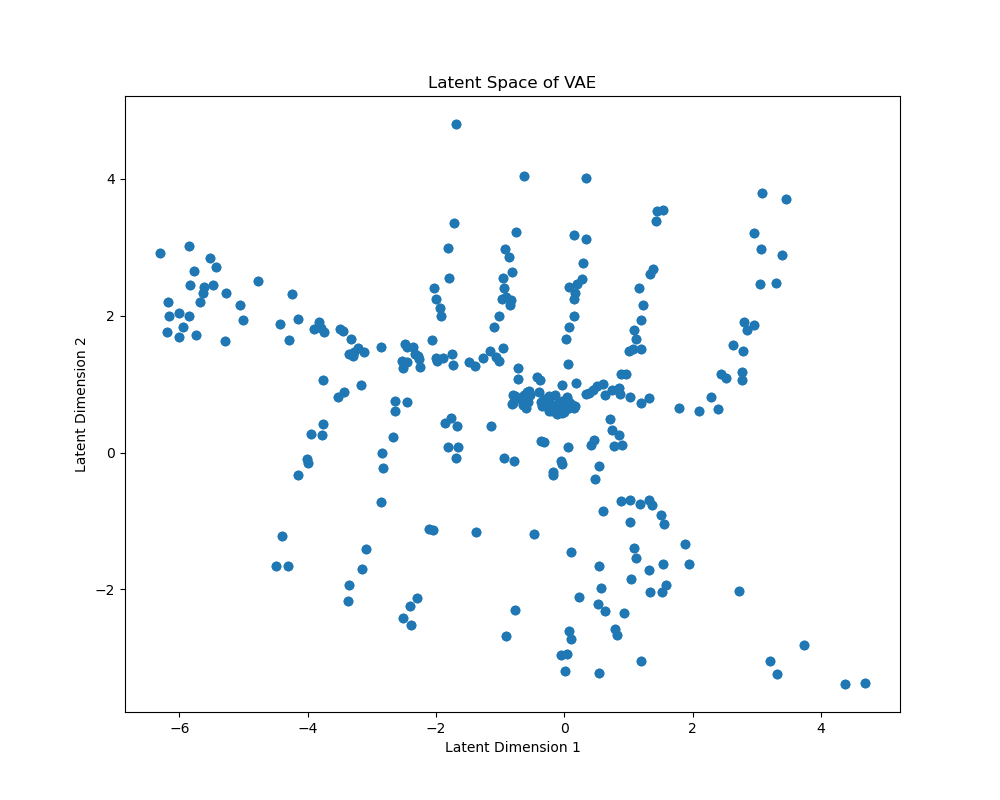
\includegraphics[width=0.45\textwidth]{images/latent_space_fire_evacuation_beta0.png}
\label{fig:beta0latent}
}
\hfill
\subfigure[Latent space \(\beta=1\)]{
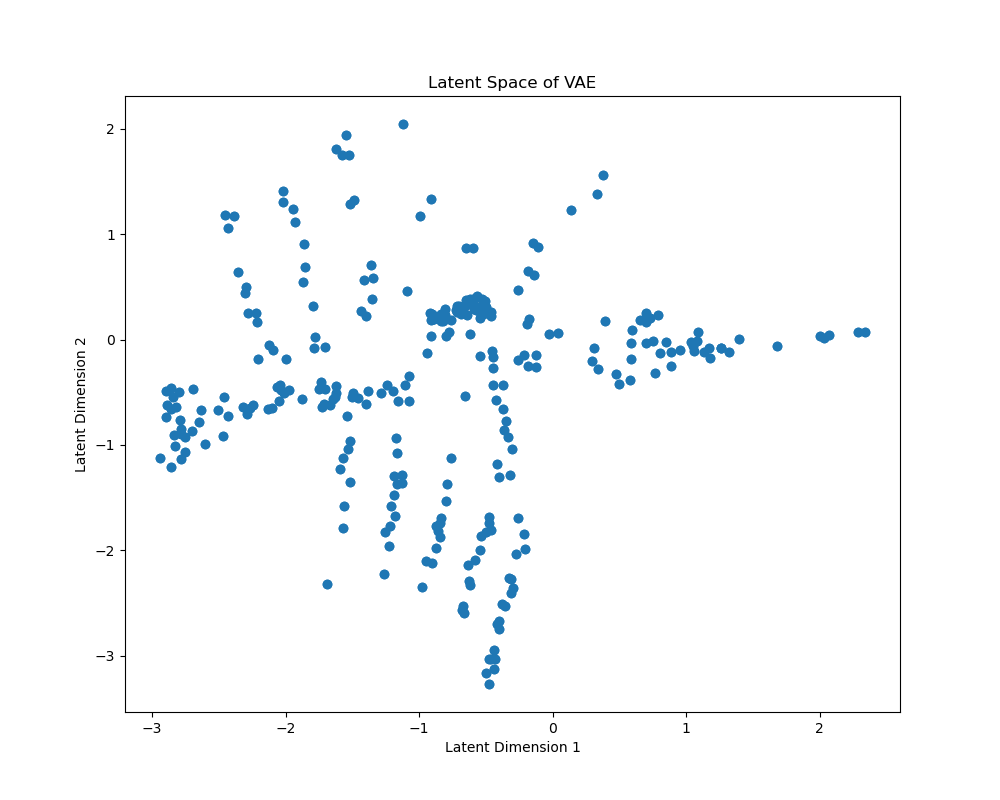
\includegraphics[width=0.45\textwidth]{images/latent_space_fire_evacuation_beta1.png}
\label{fig:beta1latent}
}
\caption{Latent space for\(\beta\) Values}
\label{fig:betalatent}
\end{figure}

\paragraph{1000 generated samples}
Next, we plan to use the decoders from the models trained with three different \(\beta\) values to generate data points. To determine the numerical range to input into the encoder, we aim to understand the range of values when mapping the test dataset to the latent space. Thus, we input the test dataset into the encoder and visualize the two-dimensional latent space as a scatter plot, as depicted in Figure \ref{fig:beta1latent}. From the graph, it is evident that when the test dataset is mapped to the latent space, the horizontal and vertical coordinates fall within the ranges of (-3, 3) and (-3, 3), respectively.


Therefore, we plan to use values within this range as input to the decoder to generate 1000 data points. We employed two methods to sample the latent space: normal distribution and uniform distribution. In the case of the uniform distribution, we uniformly sampled 32 points along the \(x\)-axis in the range \([-3, 3]\), and also uniformly sampled 32 points along the \(y\)-axis in the range \([-3, 3]\). This allowed us to generate \(32 \times 32 = 1024\) samples using these two dimensions. Taking 1000 samples from this set and inputting them into the decoder resulted in the generation of 1000 synthetic data points. The generated data points are depicted in Figure \ref{fig:generate_lin_beta}.

\begin{figure*}[ht]
\centering

\subfigure[\(\beta=0\)]{
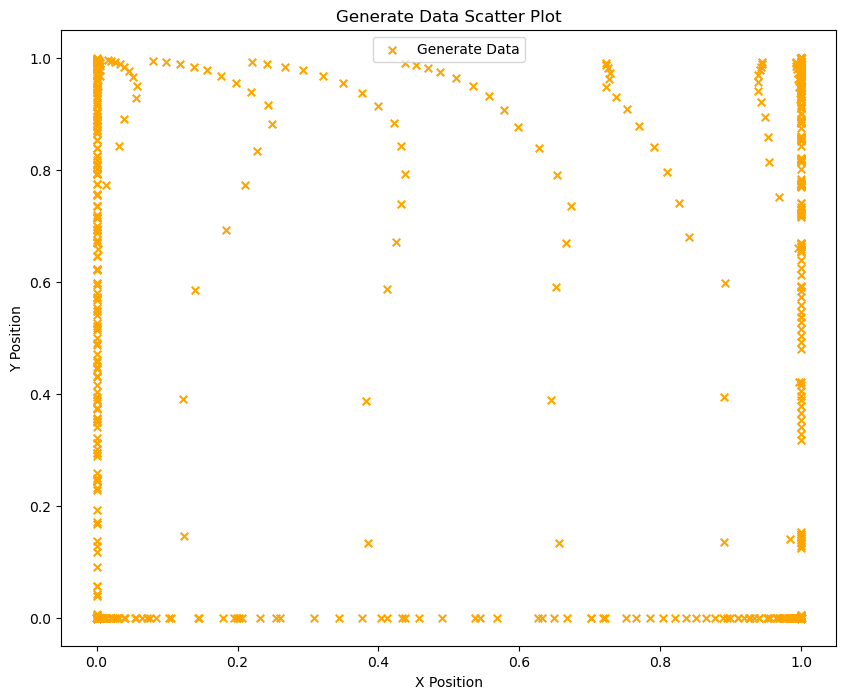
\includegraphics[width=0.3\textwidth]{images/generate_lin_beta0.png}
\label{fig:generate_lin_beta0}
}
\hfill
\subfigure[\(\beta=0.5\)]{
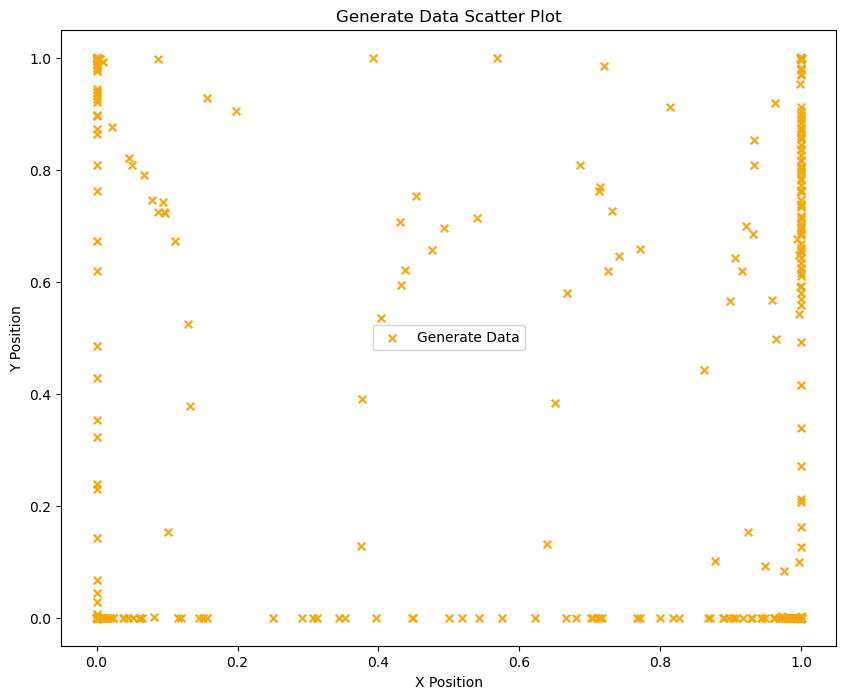
\includegraphics[width=0.3\textwidth]{images/generate_lin_beta05.png}
\label{fig:generate_lin_beta05}
}
\hfill
\subfigure[\(\beta=1\)]{
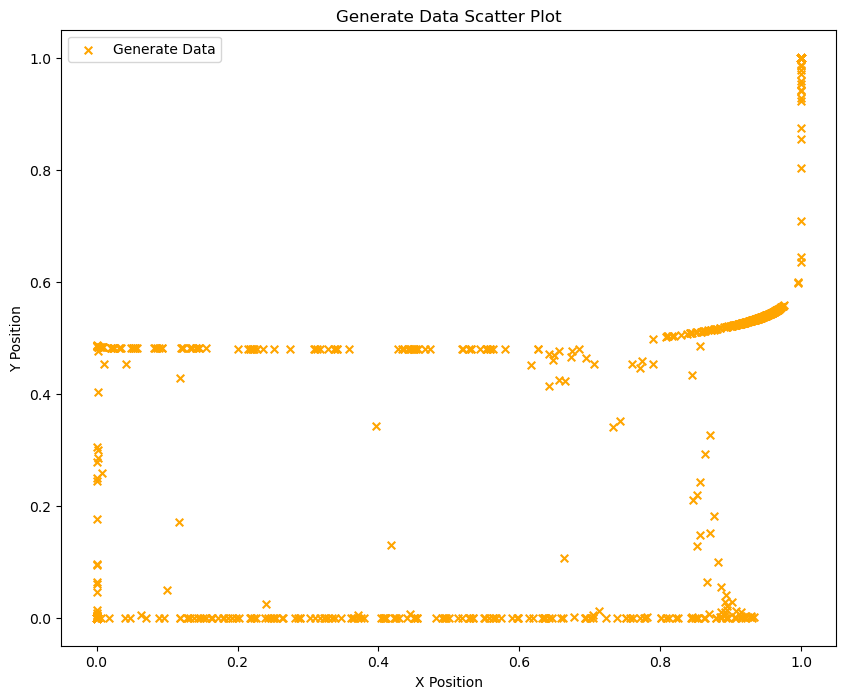
\includegraphics[width=0.3\textwidth]{images/generate_lin_beta1.png}
\label{fig:generate_lin_beta1}
}
\caption{Generated Data for Model with Different \(\beta\) Values}
\label{fig:generate_lin_beta}
\end{figure*}

Based on the previously demonstrated distribution of the latent space \ref{laten_space_fire}, we can also consider it as a normal distribution. Therefore, we adopted a Gaussian sampling approach with a mean of (-0.5, 0) and a covariance matrix of \(\begin{bmatrix}1 & 0.5\\ 0.5 & 1\end{bmatrix}\) to sample 1000 points. Subsequently, these samples are used to generate data, and the final generated results are depicted in Figure \ref{fig:generate_normal_beta}.

\begin{figure*}[ht]
\centering

\subfigure[\(\beta=0\)]{
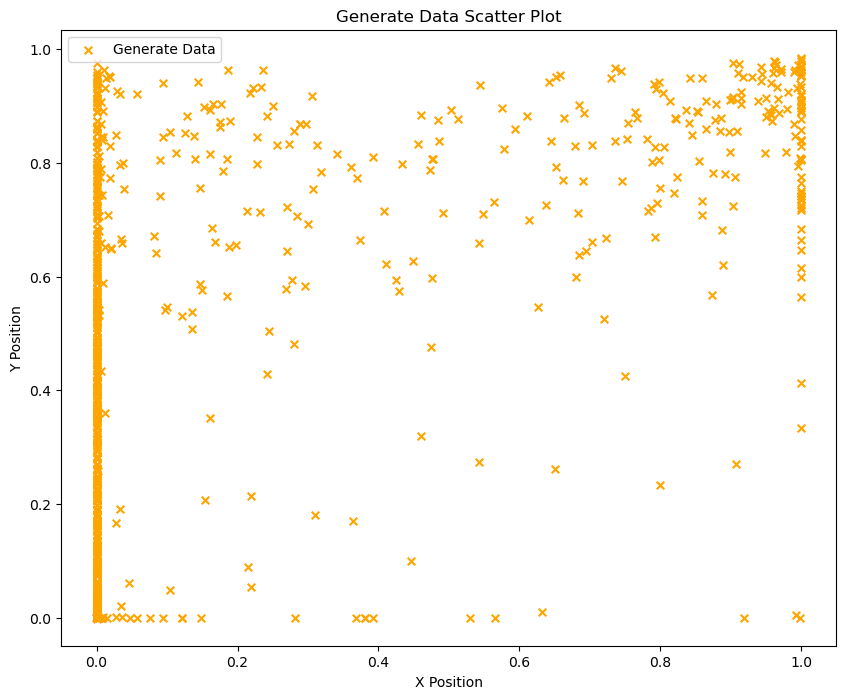
\includegraphics[width=0.3\textwidth]{images/generate_normal_beta0.png}
\label{fig:generate_normal_beta0}
}
\hfill
\subfigure[\(\beta=0.5\)]{
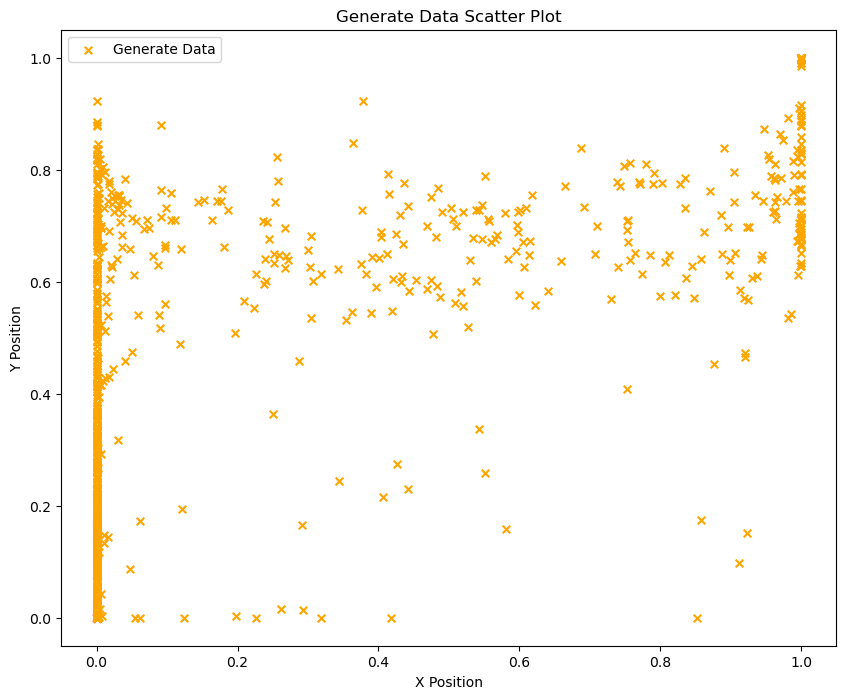
\includegraphics[width=0.3\textwidth]{images/generate_normal_beta05.png}
\label{fig:generate_normal_beta05}
}
\hfill
\subfigure[\(\beta=1\)]{
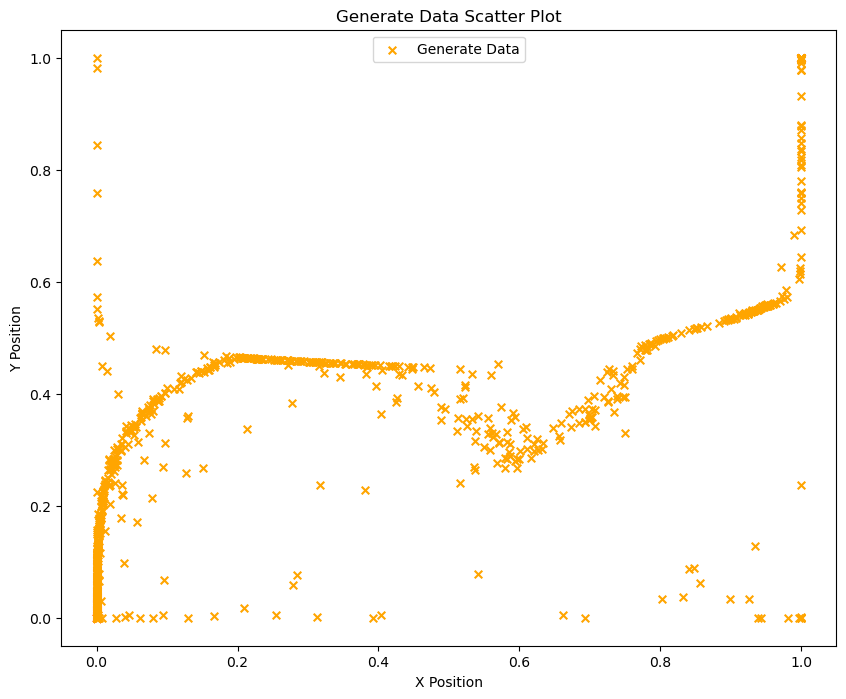
\includegraphics[width=0.3\textwidth]{images/generate_normal_beta1.png}
\label{fig:generate_normal_beta1}
}
\caption{Generated Data for Model with Different \(\beta\) Values}
\label{fig:generate_normal_beta}
\end{figure*}

The models can somewhat reconstruct the test data. But from the generated data shown above, we observe that the models' ability to generate data is quite poor. Because we can hardly find patterns among them that resemble those present in the original data points. We speculate that the reason for this might be the insufficient quantity of training data or the model's inability to capture this particular pattern

\paragraph{Critical Number Estimation}
Since the previous models are unable to generate patterned data similar to that found in the FireEvac dataset, a team member of us attempted to build a new VAE model independent of Task 3, and making numerous attempts. Various experiments were conducted, including trying different \(\beta\) values, hidden layer numbers, latent space dimensions, hidden layer neuron numbers, and activation functions. However, none of the models trained from these attempts are able to generate reliable data. Using such data for evaluation would be irresponsible concerning the safety of people inside buildings. Therefore, we prefer not to use data generated by this method for evaluating the critical number at the main entrance. Instead, we will rely on the dataset to assess the critical number at the main entrance.

Our strategy is as follows: We will start by merging the training and test sets of FireEvac. In our experiments, we generate one person at a time, and their location data is randomly selected uniformly from the merged dataset. The diagrams in Figure \ref{pedestrian} illustrate the scenarios when 50 people are generated and when a count of 90 pedestrians has been reached, respectively. 

\begin{figure*}[ht]
\centering

\subfigure[50 people generated]{
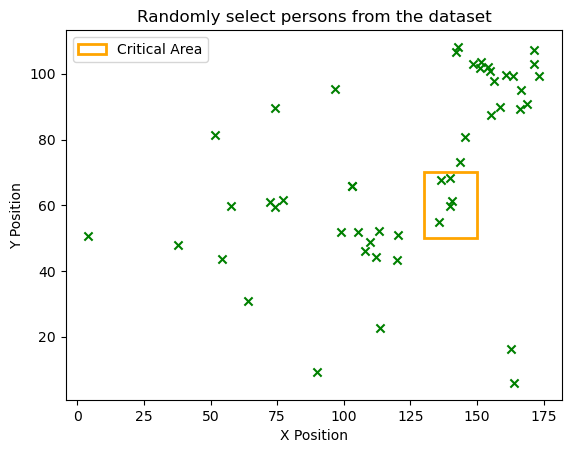
\includegraphics[width=0.45\textwidth]{images/pedestrians50.png}
\label{pedestrian50}
}
\hfill
\subfigure[90 people generated]{
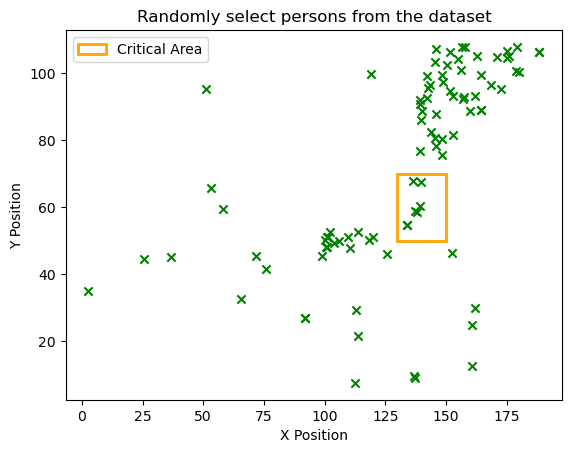
\includegraphics[width=0.45\textwidth]{images/pedestrians90.png}
\label{pedestrian90}
}
\caption{Randomly select persons from the dataset}
\label{pedestrian}
\end{figure*}

If the generated pedestrian is located at the sensitive area in front of the main entrances, we increment the counter. When the count accumulates to 100, which is the Critical Number, we record how many people have been generated in total. Figure \ref{pedestrian1032} illustrates the scenario when the critical area reaches 100 people, at which point a total of 1032 people have been generated.
\begin{figure}
\centering
    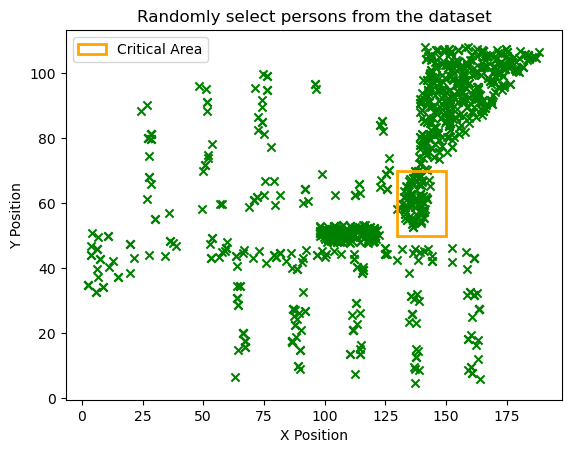
\includegraphics[width=0.6\textwidth]{images/pedestrians1032.png}
    \caption{Critical area with 100 People}
    \label{pedestrian1032}
\end{figure}

To accurately estimate the number of peoples in the sensitive area in front of the main entrance that typically exceeds the critical number under such a distribution, we repeated the above experiment one hundred thousand times. We then calculated the average and median of these one hundred thousand runs. Their respective values are 1249.6 and 1246.0. In other words, when the number of peoples inside the building approaches about 1246, it reaches the critical number for the MI building.


\paragraph{Questions from the first page of the exercise sheet}
Since the VAE has already been implemented in Task 3, we are not including the time spent here. However, it is evident that the generated data is not ideal. Both of our team members collectively spent approximately 35 hours testing and refining the model in an attempt to generate satisfactory data. Regarding the final critical number estimation, it took one hour to implement and test.

We chose not to explicitly incorporate a precision metric since the efficacy of outcomes is readily discernible through visual inspection of images. Additionally, given that the data comprises two-dimensional coordinates, its accurate representation on a flat plane inherently yields a high level of precision.

In this task, we learned how to train VAEs more effectively to enhance their performance. Additionally, we recognized that while VAEs are an excellent method for generating data, their performance may suffer when there is a shortage of training data.

\paragraph{Vadere scenario for the MI building}
By observing the scattered distribution of points in the FireEvac dataset, we created a map with dimensions of $120 \times 180$. Using the \textit{source} tool in Vedere, we meticulously created a rectangle as an exit according to given coordinates. To easily identify the location of walls, we utilized the \texttt{add\_pedestrian.py} tool created in Exercise 02 to add 1200 pedestrians to the scenario, adhering to the distribution $p(x)$. This facilitated the recognition of wall positions.

After creating the walls using the \textit{Obstacle} tool, the previously generated 1200 pedestrians were removed. Subsequently, we used \texttt{add\_pedestrian.py} again to reintroduce 100 pedestrians into the scenario, following the distribution $p(x)$. Thus, the scenario was successfully created. The visualization can be seen in Figure \ref{mi_building_vedere}. The process of adding pedestrians has been documented in the \texttt{add\_pedestrian\_with\_distribution.ipynb} file.

After successfully setting up the scenario, we tried running it through the GUI. However, we notice that each time we ran the scenario, the GUI display turned gray, which initially led us to suspect it might be due to an excessive number of pedestrians. Yet, after a wait, the movement of pedestrians became visible. Once the paths were completed, several files were generated and stored in the designated folder. We move the folder into the project directory for further examination. 
The paths of pedestrians can be observed in the graph \ref{mi_building_vedere}. The paths taken by pedestrians do not surprise us and are consistent with the behaviour of the people we see daily on the TUM campus.

\begin{figure*}[ht]
\centering

\subfigure[start]{
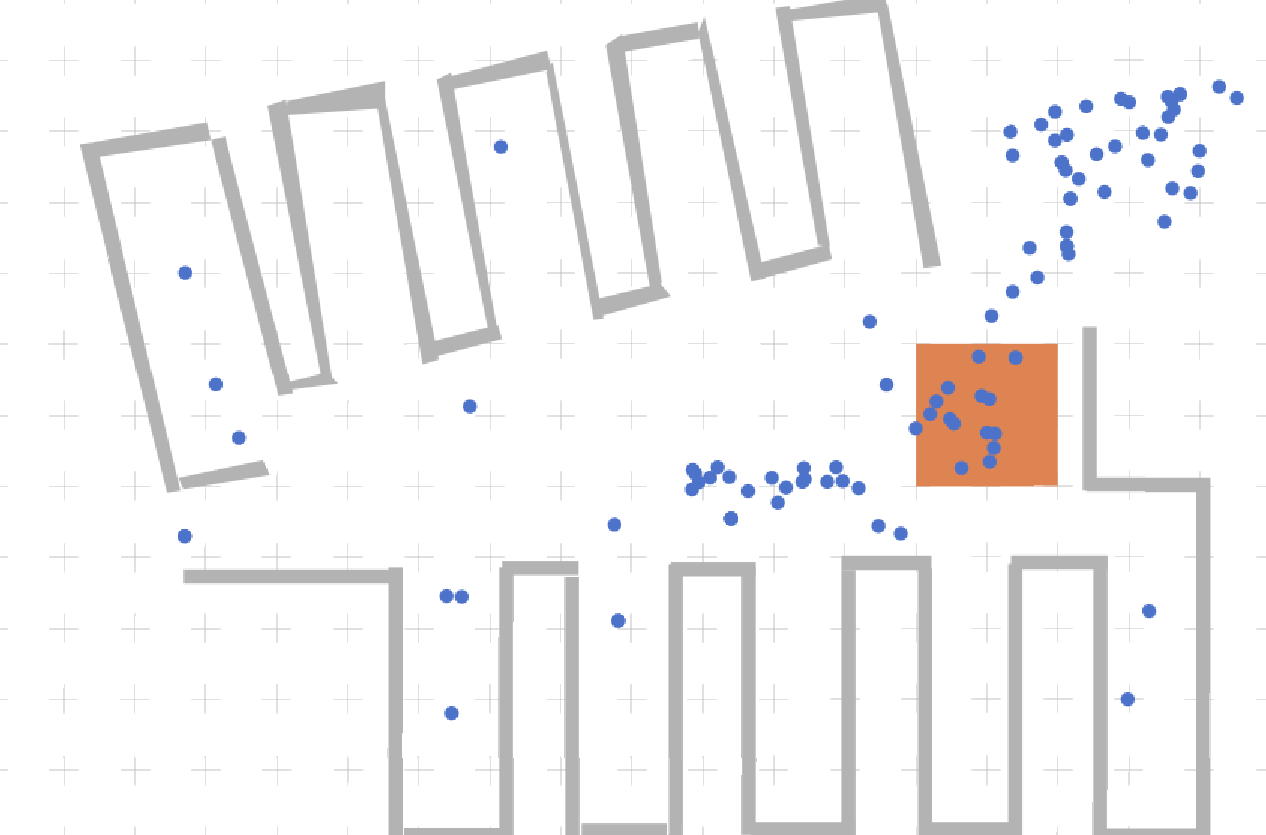
\includegraphics[width=0.3\textwidth]{images/mi_building_vedere.png}

}
\hfill
\subfigure[progress 1]{
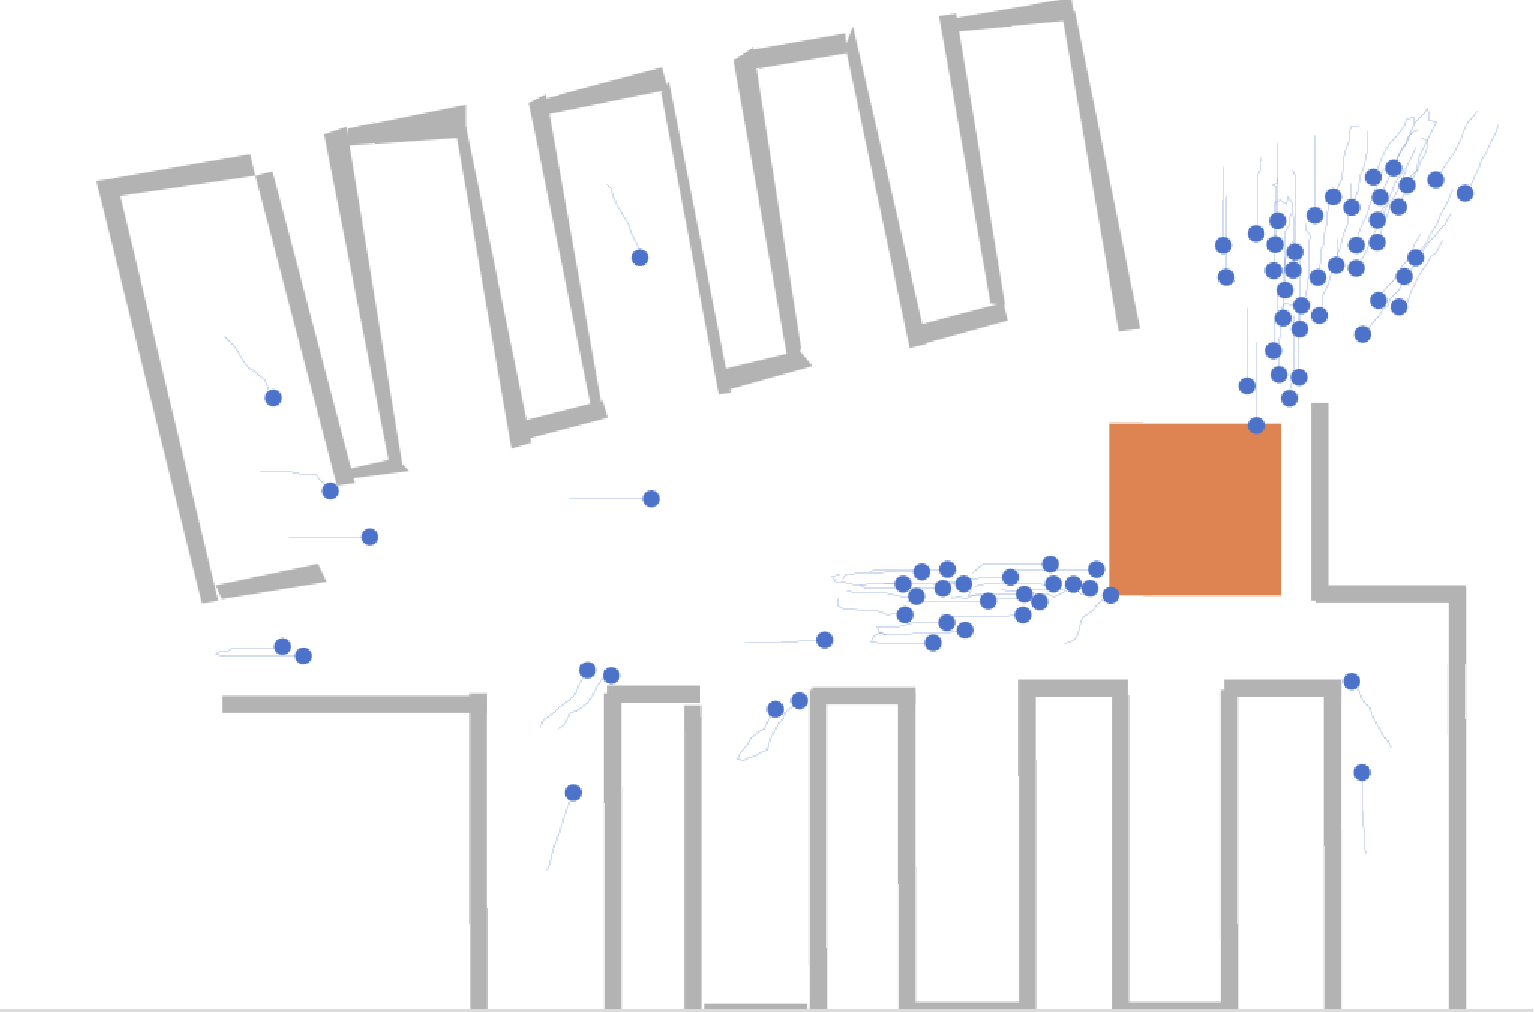
\includegraphics[width=0.3\textwidth]{images/mi_building_vedere1.png}

}
\hfill
\subfigure[progress 2]{
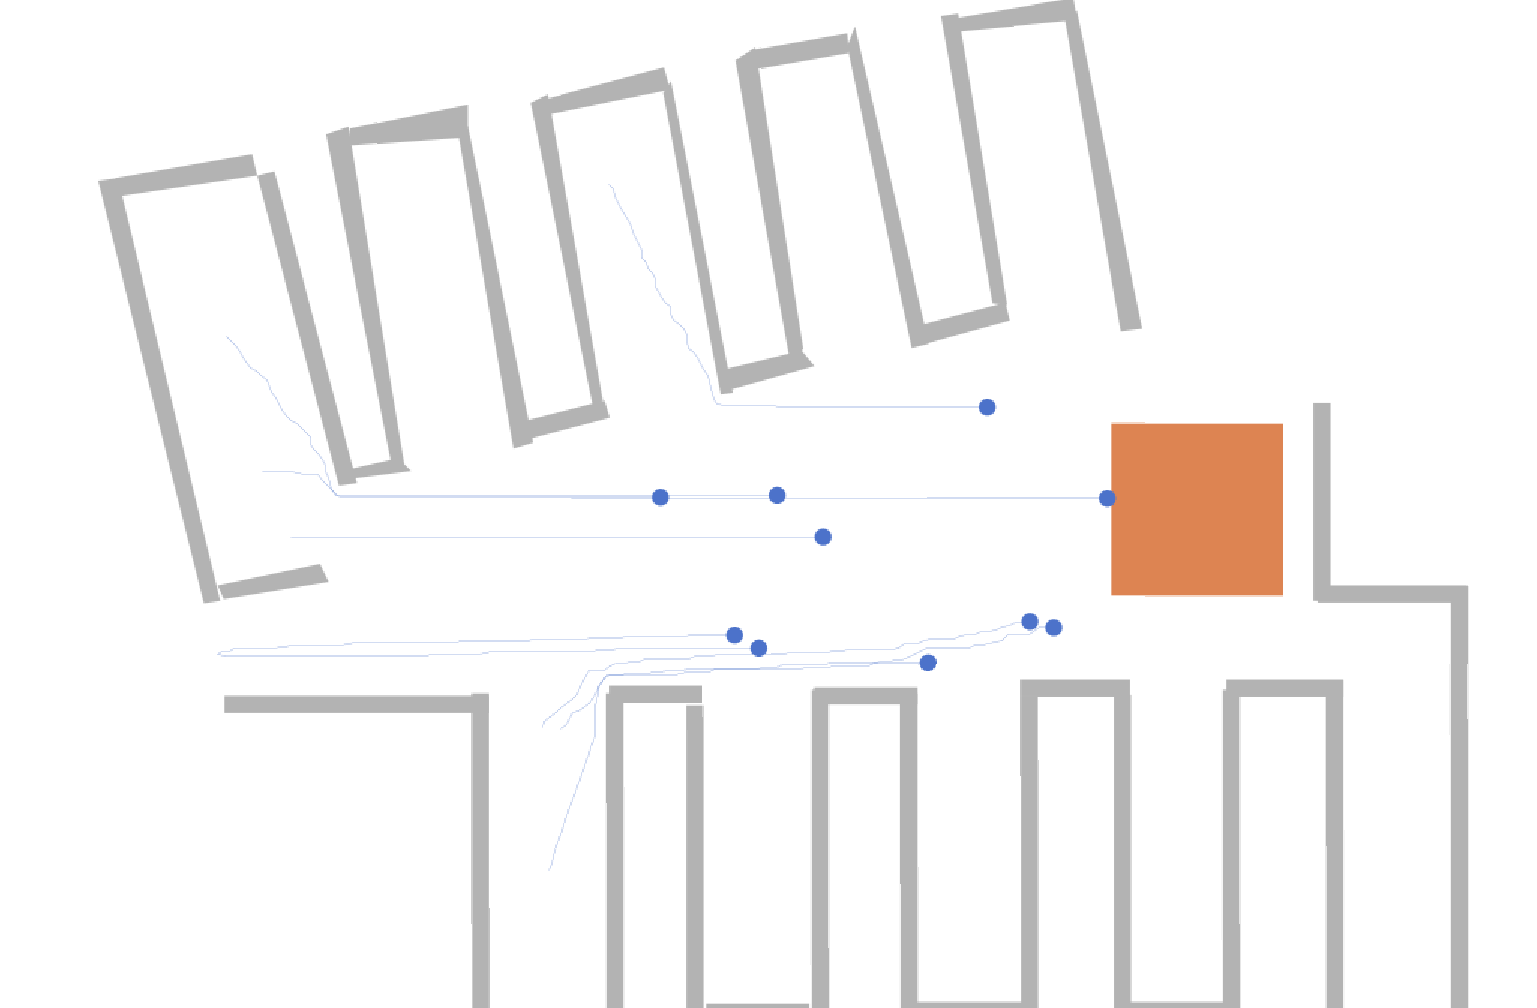
\includegraphics[width=0.3\textwidth]{images/mi_building_vedere2.png}

}
\caption{MI building scenario in Vadere}
\label{mi_building_vedere}
\end{figure*}



\end{task}